\chapter{Related Work}
\begin{figure}
	\noindent
	\makebox[\textwidth]{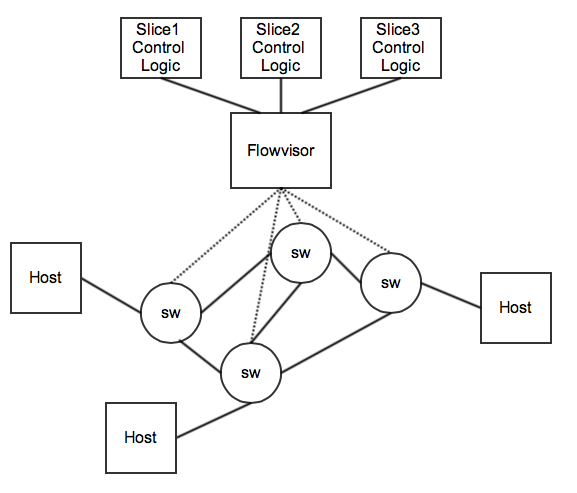
\includegraphics[width=12cm]{Figures/flowvisor.png}}%
	\caption{Flowvisor Architecture}
\end{figure}
One of our biggest motivations comes from Flowvisor \cite{flowvisor}, which slices the network hardware by placing a layer between the control plane and the data plane. Using  Flowvisor, we can split the network traffic into slices, and each slice can have its control logic. Using this, we can build a network testbed that is embedded in the physical network. \\
Flowvisor allows network researchers to test new protocols on production networks. It provides isolation between slices, so changes in one slice's control logic will not affect the other slices. Figure 3.1 illustrates the Flowvisor architecture. \\

Another work in this area is FlowN \cite{flown}, which deals with scalable Network Virtualization in software-defined networks. FlowN allows every tenant to run its own controller. The controllers are virtualized, so that the tenants' traffic are handled by the respective controller. For scalability purposes, FlowN uses databases to store the \emph{virtual-to-physical topology mappings}, thus capitalizing the years of research to achieve durable state and a highly scalable system.
